\section{Zmiana obszaru działania}

Zmiana obszaru działania to kolejna funkcjonalność umożliwiająca doprecyzowanie zleceń, które wykonawcy mają dostawać. Obszar ten zapewnia ograniczenie przydzielanych zleceń jedynie do tych, których realizacja ma się odbyć wewnątrz niego. Pozwala to odfiltrować te, które nie mogą zostać wykonane z uwagi na zbyt duże odległości. 

\pagebreak

% W stworzonym rozwiązaniu przyjęto, że obszar działania jest kołem. Powodem tego jest możliwość jego prostego zdefiniowania. Wystarczą do tego jedynie dwa parametry: centralna lokalizacja oraz promień.

Przyjęcie obszaru działania w postaci koła wymagało decyzji, czy jego promień ma być ograniczony górną granicą. Postanowiono ją wprowadzić, ponieważ zmniejsza to negatywny wpływ, jaki mogą wywierać na system nieodpowiednio korzystające z niego osoby. Mogłyby one, będące wykonawcami, wyrazić chęć świadczenia wszystkich usług na terenie całego kraju. W ten sposób zyskają dostęp do wszystkich zleceń i możliwość zgłaszania się do nich. Problem pojawia się, gdy zaczną to robić bez chęci realizacji. Aby temu zjawisku przeciwdziałać, maksymalny promień obszaru działania ograniczono do 50 kilometrów. Uznano, że jest to wartość wystarczająca dla zdecydowanej liczby prawidłowo używających systemu wykonawców.

% W tworzonym rozwiązaniu założono, że wykonawcy będą otrzymywać jedynie te zlecenia, których wykonanie ma się odbyć w obrębie określonego przez nich wcześniej obszaru działania. Postanowiono również, że wspomniany obszar działania będzie kołem, które można określić przy pomocy centralnej lokalizacji oraz promienia.

\begin{figure}[ht]
  \captionsetup[subfigure]{justification=centering}
  \centering
  \begin{subfigure}{0.32\textwidth}
    \centering
    \fbox{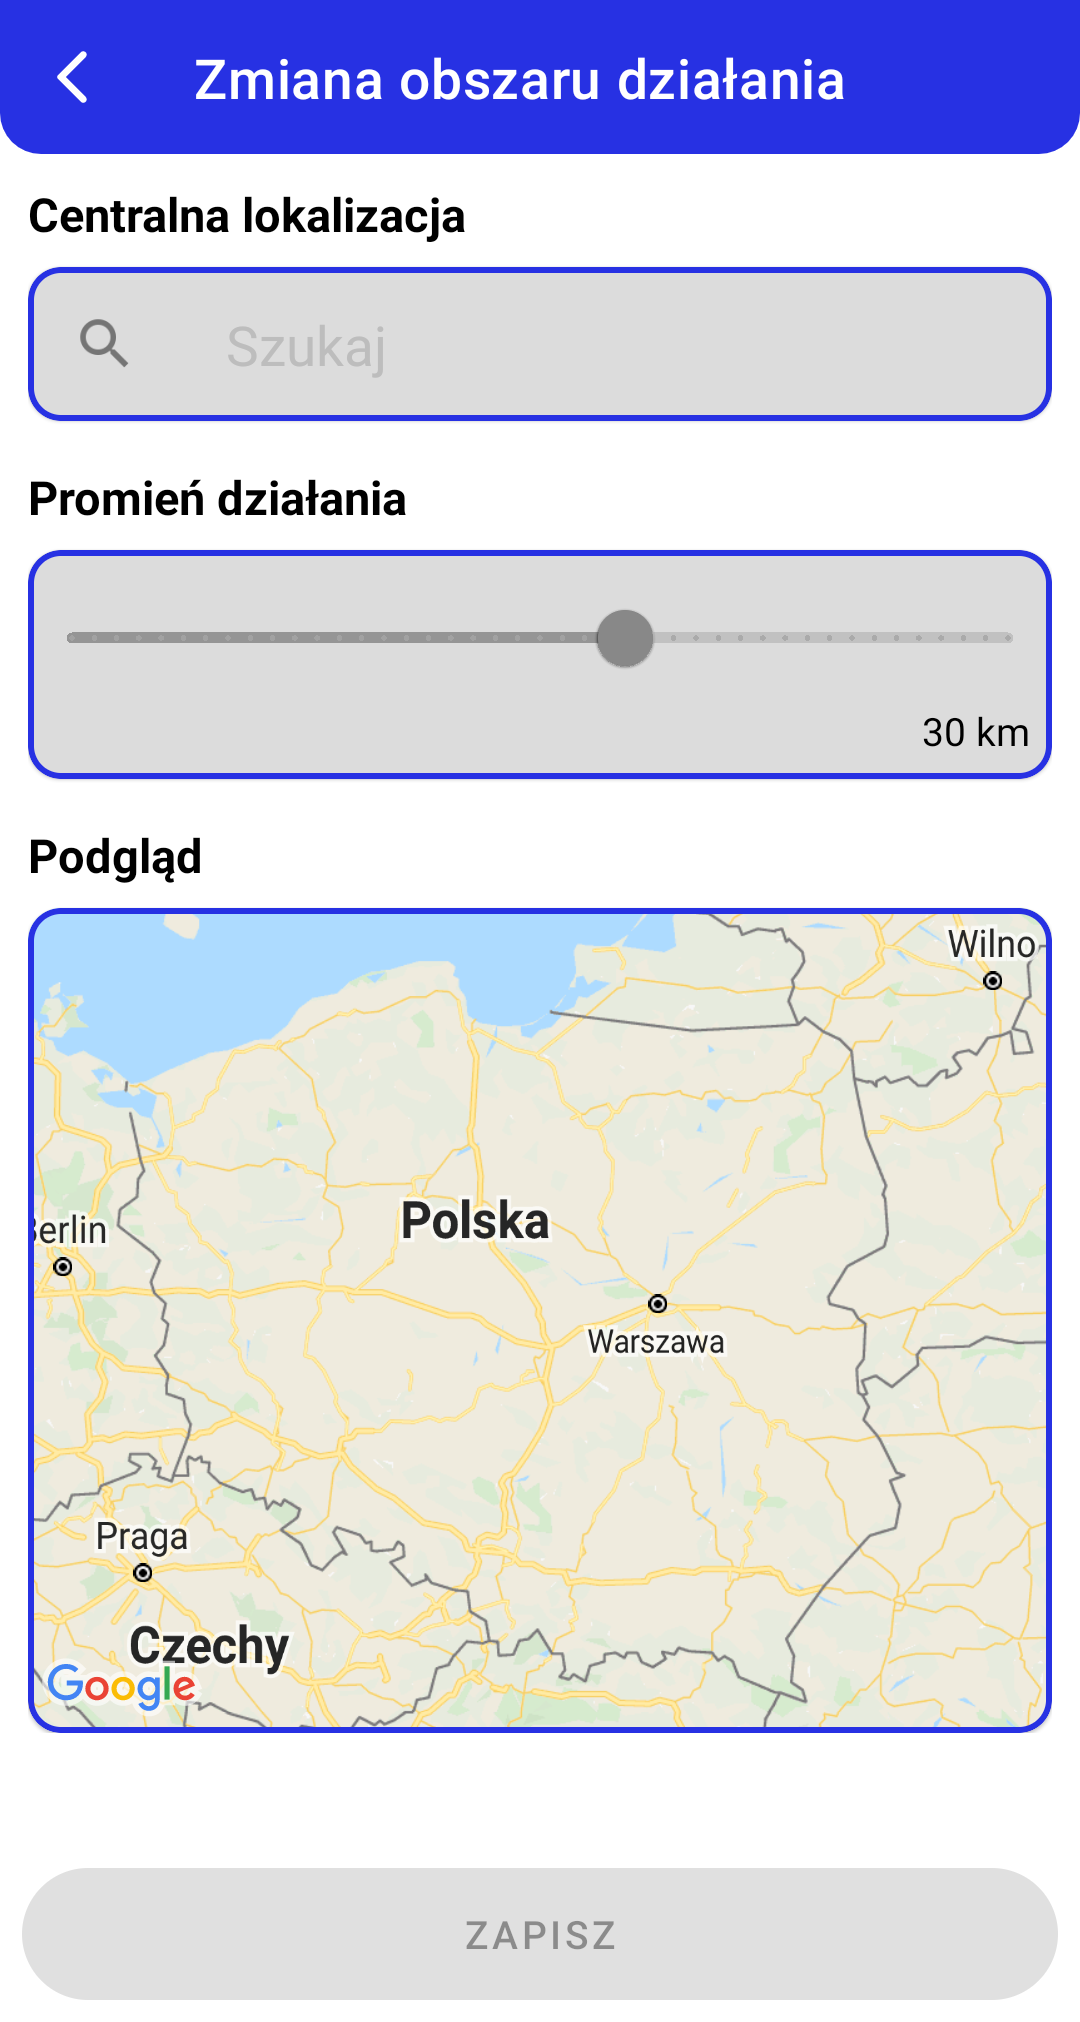
\includegraphics[width=0.97\linewidth]{screens/location_empty.png}}
    \caption{Widok nieokreślonego obszaru działania}
  \end{subfigure}
  \begin{subfigure}{0.32\textwidth}
    \centering
    \fbox{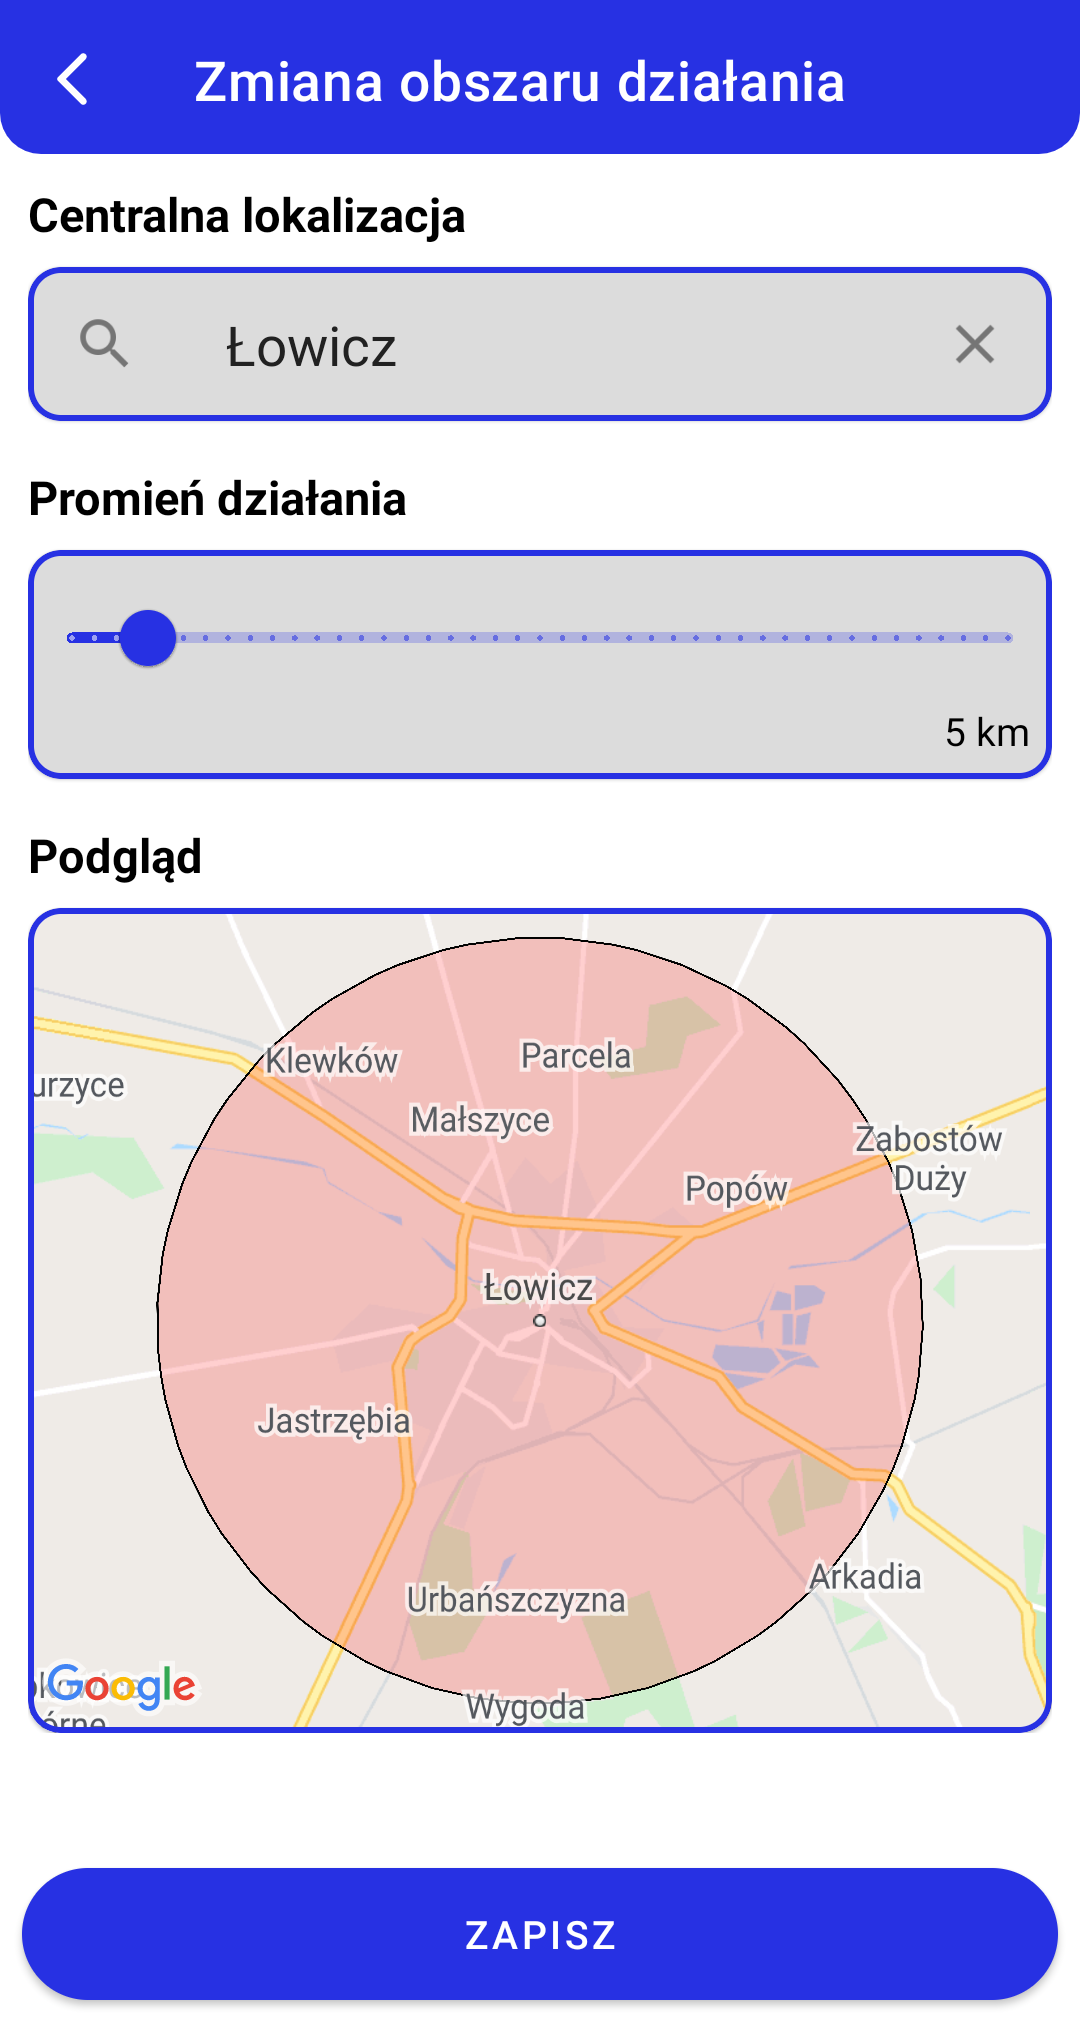
\includegraphics[width=0.97\linewidth]{screens/location_filled.png}}
    \caption{Widok określonego obszaru działania}
  \end{subfigure}
  \begin{subfigure}{0.32\textwidth}
    \centering
    \fbox{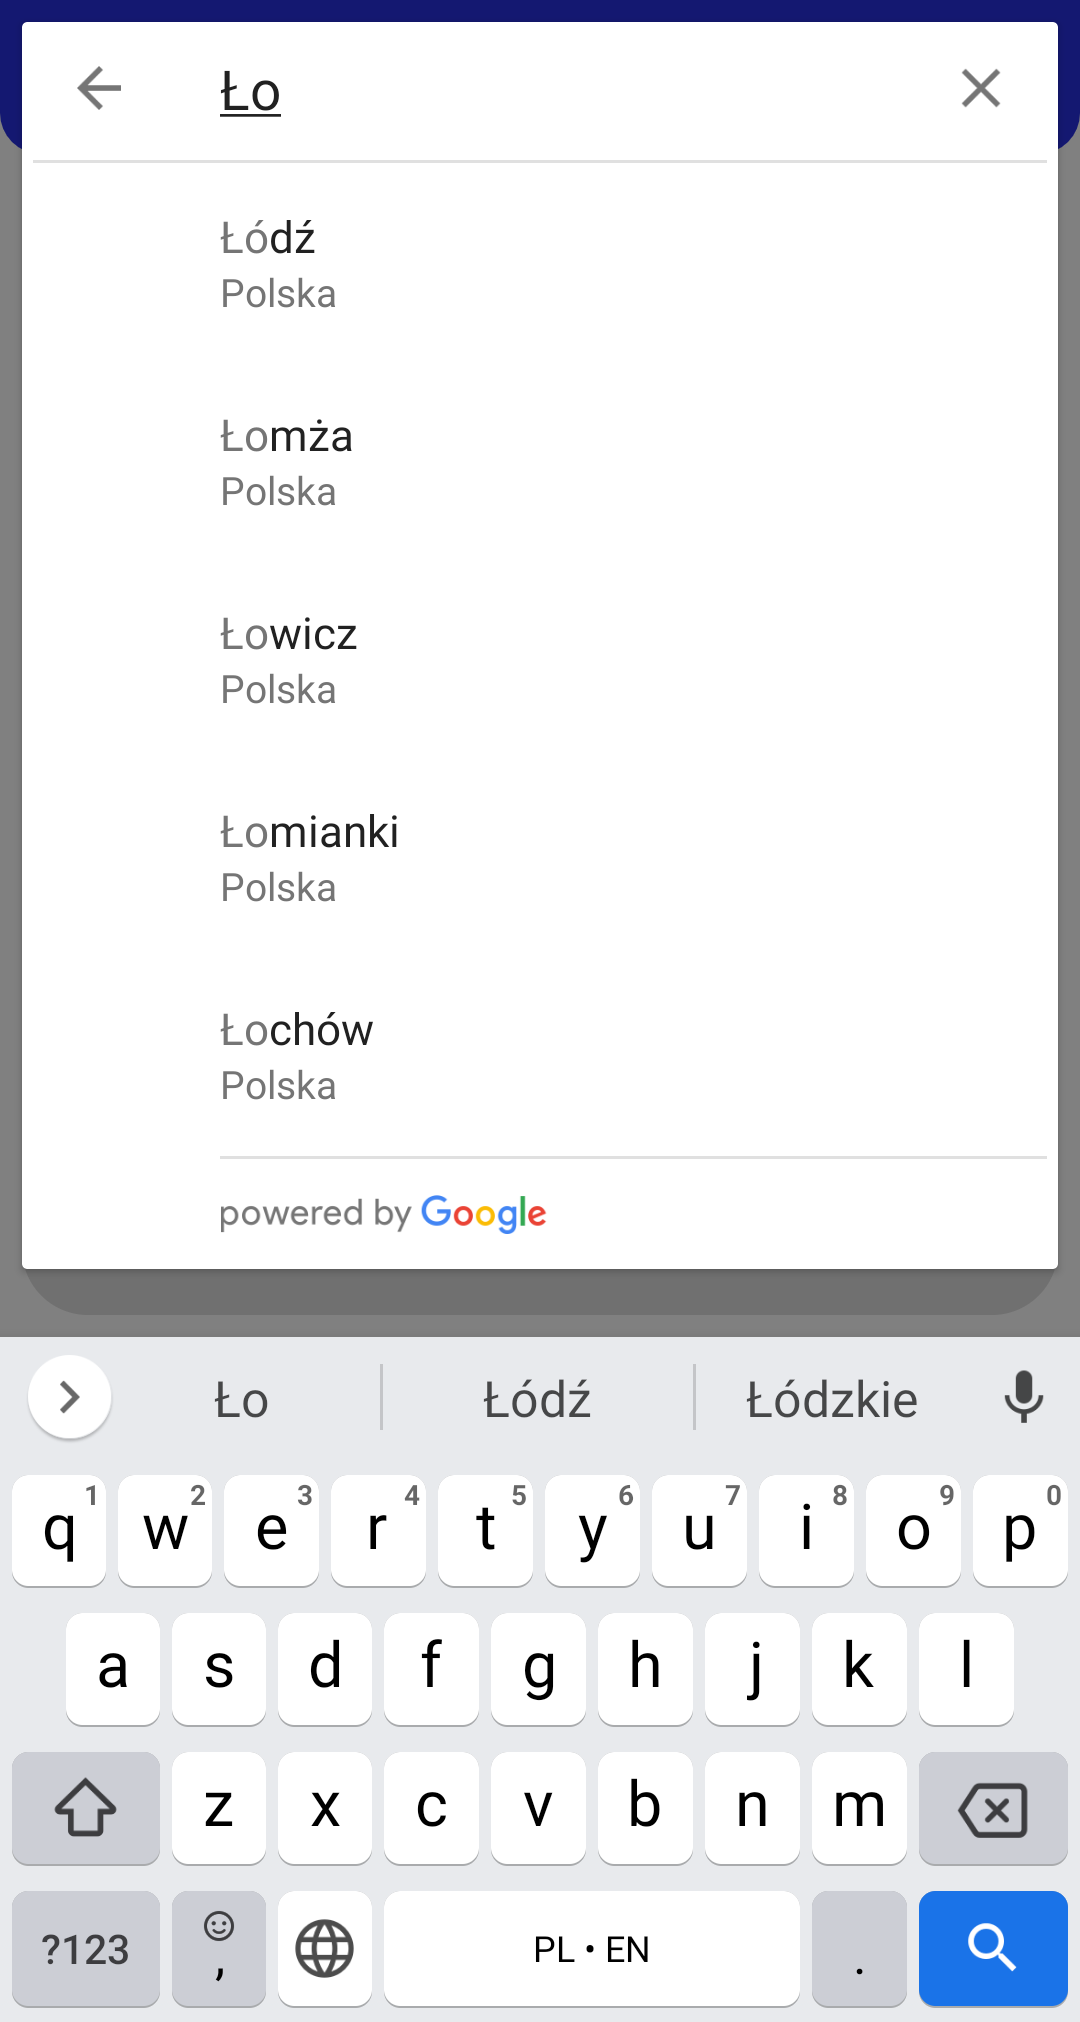
\includegraphics[width=0.97\linewidth]{screens/location_city.png}}
    \caption{Widok wyboru centralnej lokalizacji}
  \end{subfigure}
  \caption{Ekran zmiany obszaru działania}
  \label{fig:location}
\end{figure}

% Na rysunku \ref{fig:location} przedstawiony został ekran, który umożliwia zmianę lokalizacji wykonawcy. Składa się on z kontrolek umożliwiających określenie centralnej lokalizacji i promienia oraz podglądu, który te informacje wizualizuje. Wybór lokalizacji ograniczony jest do polskich miejscowości, a promienia do ustalonych 50 kilometrów.

Podczas implementacji wykorzystana została platforma Google Maps Platform i składające się na nią produkty Maps oraz Places. Umożliwiły one osadzenie mapy wewnątrz aplikacji, dostarczyły komponent wyboru lokalizacji oraz zapewniły geokodowanie, które wykorzystano wewnątrz Firebase Functions w celu walidacji poprawności lokalizacji. 